\newpage
\section{Homepage}

La schermata principale dell'applicazione appare come mostrato nella figura sottostante:

\label{Homepage}
\begin{figure}[H]
	\centering
	\fbox{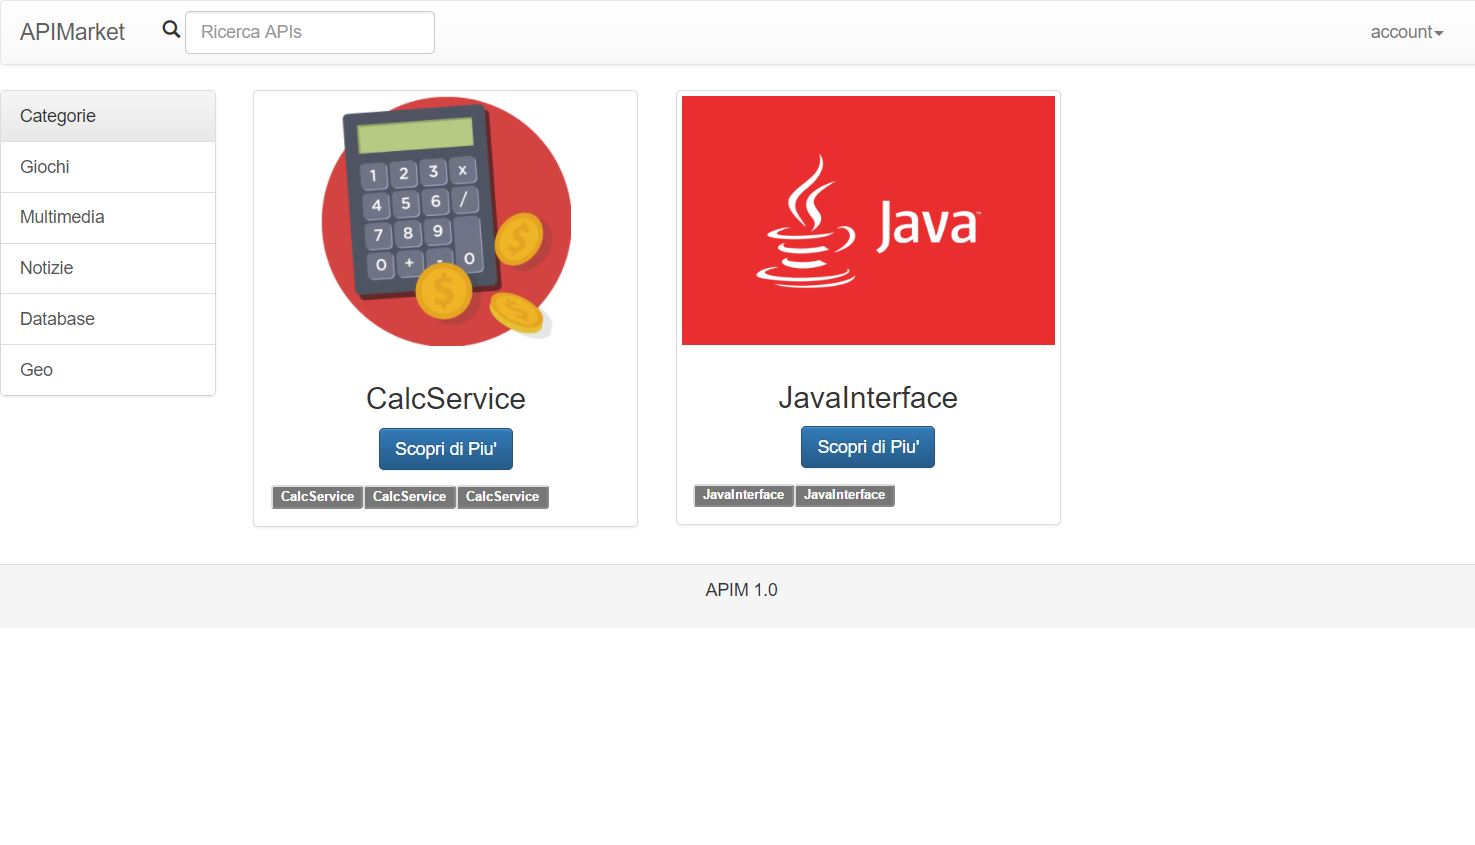
\includegraphics[scale=0.50]{img/APIM_home.JPG}}
	\caption{Homepage}
\end{figure}


Dalla schermata principale sono possibili le principali funzionalità dell'utente non autenticato. L'utente può registrarsi e autenticarsi tramite il menu in alto a destra, mentre a sinistra può sfogliare le varie categorie di API esposte nel market. Tramite la barra di ricerca, posta alla destra del logo del market, può effettuare una ricerca tramite keyword. Nella parte centrale dell'immagine sono disponibili le ultime otto API inserite all'interno dell'API Market.
In fondo alla pagina è presente il footer, che contiene alcune informazioni sull'API Market.
Come è possibile notare nella Figura 2, per la homepage, come per il resto della piattaforma è stato scelto un layout minimale e semplice per renderlo di facile utilizzo a diverse tipologie di utente.



